\documentclass[notoc, symmetric, nobib, nols]{towcenter-guideto-book}

\hypersetup{colorlinks, hyperfootnotes=true}% uncomment this line if you prefer colored hyperlinks (e.g., for onscreen viewing)

%uncomment to remove hyperlinks for Lulu upload
%\hypersetup{draft}

% creating an "ignore" command to deal with emdash problem \& comments in general
\newcommand{\ignore}[1]{}
\widowpenalty=10000

\usepackage[T1]{fontenc}
\usepackage[at]{easylist}
%\usepackage[utf8]{inputenc}
\usepackage{textcomp}
\usepackage[american]{babel}
\usepackage[autostyle]{csquotes}
\usepackage{endnotes}
\usepackage[strict]{changepage}
\usepackage{enumitem}
\setlist{noitemsep}
\usepackage{wrapfig}

\usepackage[notes15,strict,backend=biber,autolang=other,%
bibencoding=latin1,notetype=endonly,ibidtracker=constrict]{biblatex-chicago}
\bibliography{CrowdsourcingCitations}
%\addbibresource{ChatAppsReadings.bib}
\usepackage{ifthen}
\usepackage{setspace}

\renewcommand*{\biburlsetup}{%
  \Urlmuskip=0mu plus 2mu\relax
  \mathchardef\UrlBreakPenalty=200\relax
  \mathchardef\UrlBigBreakPenalty=100\relax
  \mathchardef\UrlEmergencyPenalty=9000\relax
  \appto\UrlSpecials{%
    \do\0{\mathchar`\0\penalty\UrlEmergencyPenalty}%
    \do\1{\mathchar`\1\penalty\UrlEmergencyPenalty}%
    \do\2{\mathchar`\2\penalty\UrlEmergencyPenalty}%
    \do\3{\mathchar`\3\penalty\UrlEmergencyPenalty}%
    \do\4{\mathchar`\4\penalty\UrlEmergencyPenalty}%
    \do\5{\mathchar`\5\penalty\UrlEmergencyPenalty}%
    \do\6{\mathchar`\6\penalty\UrlEmergencyPenalty}%
    \do\7{\mathchar`\7\penalty\UrlEmergencyPenalty}%
    \do\8{\mathchar`\8\penalty\UrlEmergencyPenalty}%
    \do\9{\mathchar`\9\penalty\UrlEmergencyPenalty}}%
  \def\UrlBreaks{%
    \do\.\do\@\do\/\do\\\do\!\do\_\do\|\do\;\do\>\do\]\do\)\do\}%
    \do\,\do\?\do\'\do\+\do\=\do\#\do\$\do\&\do\*\do\^\do\"}%
  \def\UrlBigBreaks{\do\:\do\-}}
\usepackage{url}
%\setcounter{biburllcpenalty}{7000}
%\setcounter{biburlucpenalty}{8000}
\urlstyle{rm}
\appto\bibsetup{\sloppy}
%\appto\biburlsetup{\Urlmuskip=0mu plus 4mu\relax}
\setlength{\dimen\footins}{9.5in}
\renewcommand{\notesname}{}


\geometry{a5paper,left=0.6in,right=0.6in,top=0.6875in,headsep=\baselineskip,
textwidth=4.4in,textheight=6.83in,headheight=\baselineskip,marginparwidth
=.1in, marginparsep=0.1in}
%\geometry{a5paper,left=13mm,top=15mm,headsep=1\baselineskip,textwidth=
%122mm,textheight=185mm,headheight=\baselineskip,marginparwidth=10mm,
%marginparsep=5mm}
%%
% Adding setspace to tighten leading on margin notes
\usepackage{setspace}

%%
% Adding back marginnote functionality that I've stripped from tufte-common.def in the process of creating towcenter-common.def
\usepackage{marginnote}
\renewcommand{\marginnote}[1]{{\marginpar{\raggedright\footnotesize
\setstretch{1.025}%
#1}}}

%%
% Setting the footnote style to roman numerals in this case
\renewcommand{\thefootnote}{\roman{footnote}}

% more on bullet positioning: http://tex.stackexchange.com/questions/78167/indentation-within-an-itemized-list
% \setlist[itemize,1]{leftmargin=\dimexpr 26pt-.5in}


%%
% Resetting the footnote counter every page for clarity (I think)
%\usepackage{perpage} %the perpage package
%\MakePerPage{footnote} %the perpage package command

%%
% Resetting footnote counters every section?!
\makeatletter
\@addtoreset{footnote}{section}
\makeatother



%%
% Book metadata
\title{Sample Tow Center printed report}
\author{Susan E. McGregor - susanemcg}
\publisher{Tow Center for Digital Journalism}


% use fontspec package and set titles to Georgia
\usepackage{fontspec}
\newfontfamily\titlefont{Times}
\newfontfamily\towknightfont{News Gothic MT}
%\newfontfamily\bodyfont{Caslon Regular}
\newfontfamily\frankmedium{Franklin Gothic Medium}
%\newfontfamily\frankregular{Franklin Gothic Regular}
%\newfontfamily\frankdemi{Franklin Gothic Demi}

%\setmainfont{Caslon Regular}

% add color package and define appropriate blues for title page
\usepackage{color}
\definecolor{darkblue}{RGB}{30,69,132}
\definecolor{lightblue}{RGB}{154,196,219}

% framed helps with graphics
\usepackage{framed}

% suppresses names and figure numbers on graphics
\usepackage{etoolbox}
\makeatletter
\patchcmd{\@caption}
  {\noindent\csname fnum@#1\endcsname: \ignorespaces}
  {}
  {}{}
\makeatother

%%
% Just some sample text
\usepackage{lipsum}

%%
% For nicely typeset tabular material
\usepackage{booktabs}

%%
% For graphics / images
\usepackage{graphicx}
\setkeys{Gin}{width=\linewidth,totalheight=\textheight,keepaspectratio}
\graphicspath{{graphics/}}

% The fancyvrb package lets us customize the formatting of verbatim
% environments.  We use a slightly smaller font.
\usepackage{fancyvrb}
\fvset{fontsize=\normalsize}

%%
% Prints argument within hanging parentheses (i.e., parentheses that take
% up no horizontal space).  Useful in tabular environments.
\newcommand{\hangp}[1]{\makebox[0pt][r]{(}#1\makebox[0pt][l]{)}}

%%
% Prints an asterisk that takes up no horizontal space.
% Useful in tabular environments.
\newcommand{\hangstar}{\makebox[0pt][l]{*}}

%%
% Prints a trailing space in a smart way.
\usepackage{xspace}


% Prints the month name (e.g., January) and the year (e.g., 2008)
\newcommand{\monthyear}{%
  \ifcase\month\or January\or February\or March\or April\or May\or June\or
  July\or August\or September\or October\or November\or
  December\fi\space\number\year
}


% Prints an epigraph and speaker in sans serif, all-caps type.
\newcommand{\openepigraph}[2]{%
  %\sffamily\fontsize{14}{16}\selectfont
  \begin{fullwidth}
  \sffamily\large
  \begin{doublespace}
  \noindent\allcaps{#1}\\% epigraph
  \noindent\allcaps{#2}% author
  \end{doublespace}
  \end{fullwidth}
}

% Inserts a blank page
\newcommand{\blankpage}{\newpage\hbox{}\thispagestyle{empty}\newpage}

\usepackage{units}

% Typesets the font size, leading, and measure in the form of 10/12x26 pc.
\newcommand{\measure}[3]{#1/#2$\times$\unit[#3]{pc}}

% Macros for typesetting the documentation
\newcommand{\hlred}[1]{\textcolor{Maroon}{#1}}% prints in red
\newcommand{\hangleft}[1]{\makebox[0pt][r]{#1}}
\newcommand{\hairsp}{\hspace{1pt}}% hair space
\newcommand{\hquad}{\hskip0.5em\relax}% half quad space
\newcommand{\TODO}{\textcolor{red}{\bf TODO!}\xspace}
\newcommand{\ie}{\textit{i.\hairsp{}e.}\xspace}
\newcommand{\eg}{\textit{e.\hairsp{}g.}\xspace}
\newcommand{\na}{\quad--}% used in tables for N/A cells
\providecommand{\XeLaTeX}{X\lower.5ex\hbox{\kern-0.15em\reflectbox{E}}\kern-0.1em\LaTeX}
\newcommand{\tXeLaTeX}{\XeLaTeX\index{XeLaTeX@\protect\XeLaTeX}}
% \index{\texttt{\textbackslash xyz}@\hangleft{\texttt{\textbackslash}}\texttt{xyz}}
\newcommand{\towcenterbs}{\symbol{'134}}% a backslash in tt type in OT1/T1
\newcommand{\doccmdnoindex}[2][]{\texttt{\towcenterbs#2}}% command name -- adds backslash automatically (and doesn't add cmd to the index)
\newcommand{\doccmddef}[2][]{%
  \hlred{\texttt{\towcenterbs#2}}\label{cmd:#2}%
  \ifthenelse{\isempty{#1}}%
    {% add the command to the index
      \index{#2 command@\protect\hangleft{\texttt{\towcenterbs}}\texttt{#2}}% command name
    }%
    {% add the command and package to the index
      \index{#2 command@\protect\hangleft{\texttt{\towcenterbs}}\texttt{#2} (\texttt{#1} package)}% command name
      \index{#1 package@\texttt{#1} package}\index{packages!#1@\texttt{#1}}% package name
    }%
}% command name -- adds backslash automatically
\newcommand{\doccmd}[2][]{%
  \texttt{\towcenterbs#2}%
  \ifthenelse{\isempty{#1}}%
    {% add the command to the index
      \index{#2 command@\protect\hangleft{\texttt{\towcenterbs}}\texttt{#2}}% command name
    }%
    {% add the command and package to the index
      \index{#2 command@\protect\hangleft{\texttt{\towcenterbs}}\texttt{#2} (\texttt{#1} package)}% command name
      \index{#1 package@\texttt{#1} package}\index{packages!#1@\texttt{#1}}% package name
    }%
}% command name -- adds backslash automatically
\newcommand{\docopt}[1]{\ensuremath{\langle}\textrm{\textit{#1}}\ensuremath{\rangle}}% optional command argument
\newcommand{\docarg}[1]{\textrm{\textit{#1}}}% (required) command argument
\newenvironment{docspec}{\begin{quotation}\ttfamily\parskip0pt\parindent0pt\ignorespaces}{\end{quotation}}% command specification environment
\newcommand{\docenv}[1]{\texttt{#1}\index{#1 environment@\texttt{#1} environment}\index{environments!#1@\texttt{#1}}}% environment name
\newcommand{\docenvdef}[1]{\hlred{\texttt{#1}}\label{env:#1}\index{#1 environment@\texttt{#1} environment}\index{environments!#1@\texttt{#1}}}% environment name
\newcommand{\docpkg}[1]{\texttt{#1}\index{#1 package@\texttt{#1} package}\index{packages!#1@\texttt{#1}}}% package name
\newcommand{\doccls}[1]{\texttt{#1}}% document class name
\newcommand{\docclsopt}[1]{\texttt{#1}\index{#1 class option@\texttt{#1} class option}\index{class options!#1@\texttt{#1}}}% document class option name
\newcommand{\docclsoptdef}[1]{\hlred{\texttt{#1}}\label{clsopt:#1}\index{#1 class option@\texttt{#1} class option}\index{class options!#1@\texttt{#1}}}% document class option name defined
\newcommand{\docmsg}[2]{\bigskip\begin{fullwidth}\noindent\ttfamily#1\end{fullwidth}\medskip\par\noindent#2}
\newcommand{\docfilehook}[2]{\texttt{#1}\index{file hooks!#2}\index{#1@\texttt{#1}}}
\newcommand{\doccounter}[1]{\texttt{#1}\index{#1 counter@\texttt{#1} counter}}

% Generates the index
\usepackage{makeidx}
\makeindex

\begin{document}

% Front matter
\frontmatter

% r.1 blank page
\blankpage

% r.3 full title page
%\maketitle
%Using minipages to mimic existing layout for title page

%\cleardoublepage

\begin{figure}
\centering
\makebox[0pt][c]{%
\begin{minipage}[t][1\textheight]{0.2\textwidth}
\vspace{0pt}
\vfill

\includegraphics[width=.6\textwidth]{graphics/ColumbiaLogo.pdf}
\end{minipage}
\hfill
\begin{minipage}[t][1\textheight]{0.80\textwidth}
\vspace{0pt}
\begin{flushleft}

%\textcolor{darkblue}{\towknightfont{\fontsize{30}{30}\selectfont Guide to}}
\textcolor{lightblue}{\towknightfont{\fontsize{47}{47}\selectfont \textbf{Guide to}}}

\vspace{0.4in}

\textcolor{darkblue}{\textbf{\titlefont\fontsize{58}{58}\selectfont
Crowd-\\sourcing}}

\vspace{2.9in}
\textcolor{darkblue}{\towknightfont{\fontsize{16}{16}\selectfont \textbf{Mimi Onuhoa\\Jeanne Pinder\\Jan Schaffer}}}

\vspace{1.45in}

\textcolor{darkblue}{\towknightfont{\fontsize{7}{-3}\selectfont Tow Center for Digital Journalism\hspace{0.3in}Funded by the Tow Foundation and the\\[-0.08in]A Tow/Knight Guide \hspace{0.88in}James S. and John L. Knight Foundation}}
\end{flushleft}
\end{minipage}%
}%
\end{figure}



\blankpage
\blankpage
% v.4 copyright page


\null
\begin{fullwidth}
\noindent\textsf{\textbf{Acknowledgements}} \\[0.3cm]
\noindent\textit{We would like to thank the Tow Center for Digital Journalism at Columbia University for supporting our research. Emily Bell, Liz Boylan, and, in particular, Claire Wardle were an unending source of wisdom, support, common sense, and encouragement. Claire’s expertise in eyewitness media and her clear vision have been immensely valuable.  
}\\[0.1cm]\noindent\textit{
Our research also benefited greatly from the generosity of our interview subjects, who opened up their schedules and minds to tell us of their triumphs and challenges in this brave new world. To a person, they were thoughtful and candid, and we regret that we could not record every word here to mark and celebrate their contributions.  
}\\[0.1cm]\noindent\textit{
We are also grateful to those crowdsourcing experts who had already paved the way for our research---both those whom we interviewed and those we didn’t---whose work has nonetheless been instrumental in bringing this practice to where it is today.  
}\\[0.1cm]\noindent\textit{
Finally, we offer special thanks to a group of people that has unknowingly and significantly affected this report: the community members who have contributed to crowdsourcing projects, giving their time and energy to build a campaign finance database, share what they paid for medical procedures, or create a living compendium of all the people killed by police in the United States. You, community contributors, have demonstrated faith in journalists and a belief that we can work together to create journalism of great substance and meaning.
}\\[0.1cm]
\noindent\textit{\monthyear}
\end{fullwidth}
% r.5 contents
\tableofcontents


% r.7 introduction
\cleardoublepage


%%
% Start the main matter (normal chapters)
\mainmatter


\chapter{Executive Summary} 


\subsection{The Purpose of the Research}

The term “crowdsourcing” has been around for a decade. Although Wired writer Jeff Howe coined it in 2006, the ways in which news organizations define and employ it today vary enormously.

This guide is organized around a specific journalism-related definition of crowdsourcing and provides a new typology designed to help practitioners and researchers understand the different ways crowdsourcing is being used both inside and outside newsrooms. This typology is explored via interviews and case studies. 

During our research, we interviewed 51 people, analyzed 18 survey responses, engaged in online explorations of dozens of projects, and developed four in-depth case studies.

\subsection{Definition and Typologies}

\textbf{Our definition}: Journalism crowdsourcing is the act of specifically inviting a group of people to participate in a reporting task---such as newsgathering, data collection, or analysis---through a targeted, open call for input; personal experiences; documents; or other contributions.

Using that definition, most crowdsourcing generally takes two forms:
 
\begin{itemize}
\item An unstructured call-out, which is an open invitation to vote, email, call, or otherwise contact a journalist with information.\item A structured call-out, which engages in targeted outreach to ask people to respond to a specific request. Responses can enter a newsroom via multiple channels, including email, SMS, a website, or Google form. Often, they are captured in a searchable database.
\end{itemize}

We argue that crowdsourcing requires a specific call-out. If a newsroom simply harvests information or content available on the social web, we don't believe this constitutes crowdsourcing. For us, the people engaging in crowdsourcing need to feel they have agency in contributing to a news story.

We acknowledge that crowdsourcing efforts don't fit neatly into discrete classification, but for the purpose of this report, we've organized our typologies into six different calls to action: 

\begin{itemize}
\item \textbf{Voting}---prioritizing which stories reporters should tackle. 
\item \textbf{Witnessing}---sharing what you saw during a news event.
\item \textbf{Sharing personal experiences}---telling what you know about your life experience. 
\item \textbf{Tapping specialized expertise}---contributing data or unique knowledge.
\item \textbf{Completing a task}---volunteering time or skills to help create a news story.
\item \textbf{Engaging audiences}---joining in call-outs that can range from informative to playful.
\end{itemize}

\subsection{Principal Findings}  

\begin{itemize}
\item The rise of crowdsourcing correlates with the rise of the Internet and web technologies that have made it easier for journalists to identify and cultivate communities; organize data; and follow real-time, breaking-news developments.

\item Crowdsourcing leaders, like \textit{The Guardian} and ProPublica, believe in the practice and integrate it thoroughly.

\item Some stories involving specialized data or unique personal experiences can be told only via crowdsourcing. 

\item Crowdsourcing allows newsrooms to build audience entry points at every stage of the journalistic process---from story assigning, to pre-data collection, to data mining, to sharing specialized expertise, to collecting personal experiences and continuing post-story conversations.
 
\item News organizations are taking different paths toward audience growth and engagement. Some are focusing on crowdsourcing; others are interested in mining non-solicited citizen contributions through social media.

\item Good crowdsourcing efforts are high-touch, labor-intensive efforts. Journalists must determine a type of call-out, the communities to target, the method for collecting responses, and the avenues for connecting and giving back to the community of contributors. 

\item News organizations must demonstrate active engagement and reward the community during the crowdsourcing process, by actively participating in comments or updating contributors on a story's progress, to encourage more contributions.

\item Some organizations have created additional venues, such as Facebook Groups, to continue the conversation.

\item Tension exists in some news organizations around whether crowdsourced contributions are trustworthy. Experienced practitioners say this is not a problem. 

\item For digital-first startups, in particular, crowdsourcing provides a way to cultivate new audiences from scratch and produce unique journalism. 

\item Some news organizations are situating crowdsourcing out of newsrooms and within communities. 

\item Several crowdsourcing ventures are turning into bona fide businesses, offering B2B (business-to-business) crowdsourcing solutions to media companies. 

\item News consumers clearly have stories to share, but they don't necessarily want to write the news.

\item Ways of measuring the impact of engaging in crowdsourcing initiatives and analyzing its value to a newsroom are still in development. Such measures have not been institutionalized.
\end{itemize}

\subsection{Conclusion} 

The research shows that crowdsourcing is credited with helping to create amazing acts of journalism. It has transformed newsgathering by introducing unprecedented opportunities for attracting sources with new voices and information, allowed news organizations to unlock stories that otherwise might not have surfaced, and created opportunities for news organizations to experiment with the possibilities of engagement just for the fun of it.

In short, it has done just what the pundits predicted a decade ago: helped turn journalism into more of a conversation, rather than a one-way megaphone. 

Crowdsourcing also deserves credit for shaping journalism into more of an iterative process: as data or stories come in from contributors, reporters see new possibilities for their journalism---and news organizations see opportunities to incrementally publish those contributions in ways that tease out more. 

Certainly, though, crowdsourcing can be high-touch and high-energy, and not all projects work the first time. 

For all its potential, crowdsourcing's promise is widespread and systemic at just a few big news organizations---ProPublica, WNYC, and \textit{The Guardian}, for example. At other mainstream news organizations, like CNN Digital and \textit{The New York Times}, only a handful of reporters and editors---and not the institutions themselves---are the standard bearers. 

To be sure, crowdsourcing businesses are flourishing outside of journalism. But within the news industry, wider systemic adoption may depend on more than enthusiasm from experienced practitioners and accolades from sources thrilled by the outreach.  

We would like to see more research and evidence exploring whether crowdsourcing can foster greater support for journalism. That support might take the form of audience engagement, such as attention, loyalty, time spent on a site, repeat visits, or contributing personal stories. Or it might mean financial support from members or donors, from advertisers who want to be associated with the practice, or from funders who want to support it. 

Also to be explored is whether crowdsourced stories have more real-world impact, such as prompting legislative change, than other types of journalism do. 

Until this data is available and a better suite of tools and practices is developed, some news organizations may be wary of joining the ranks of long-time practitioners and investing the time and resources needed to support crowdsourcing projects



\chapter{Introduction}

When health care reporter Elisabeth Rosenthal needed to find patients for her stories, she stood in a hospital parking lot looking for the right prospects. ``It's kind of low-yield and it's cold,'' she remembered.%\autocite{Rosenthal}

But when she tackled a series for \textit{The New York Times} on the cost of U.S. medical care two years ago, she tried a new approach. “Obviously, I needed patients,” she said.
       
A simple invitation to readers on February 11, 2013, opened the door to finding sources that populated the 10 stories of her award-winning ``Paying Till It Hurts''.\autocite{Paying} She queried: ``Have you had a hip replacement? Tell us about your costs and bills.'' And 512 readers responded.

Soon, responses multiplied---addressing the costs of colonoscopies, pregnancies, emergency room visits, and more. Rosenthal tapped these street-level views to craft many of her stories. ``It really changed my view of how crowdsourcing could give you insight,'' she said.%\autocite{Rosenthal} 

Although it was not that long ago, her use of crowdsourcing---reaching out to ordinary people to capture their experiences on her subjects---was a teachable moment for \textit{The New York Times}. Rosenthal recalled that the news organization had few templates for how to frame the questions she asked or where to place them on a web page, and few tools for searching the responses. It also provoked discussion on what the policy should be for emailing and thanking contributors, and even whether to permit a public Facebook page for a growing community that wanted to stay engaged. 

Two years later, many of those issues have been resolved. Rosenthal's crowdsourcing led to the creation of a database of some 12,000 contributors that New York Times reporters can now use, and a Facebook Group with more than 6,500 members.

Her discovery of the potential for capitalizing on community experiences represents far more than an isolated event. It fits neatly into a larger trend of newsrooms' willingness to increasingly embrace the role that the crowd can play in gathering and contributing information.

\textit{Wired} writer Jeff Howe was the first to spotlight this trend in a 2006 article, wherein he anointed this kind of activity as ``crowdsourcing.''\autocite{Howe} But the ways in which news organizations have come to define and employ it since vary enormously. 

This guide is organized around a specific, journalism-related definition of crowdsourcing and articulates a new typology designed to help practitioners and researchers understand the different ways it is being used both inside and outside newsrooms. 

In exploring how crowdsourcing is evolving in the media ecosystem, we asked journalists about the kinds of jobs crowdsourcing is helping them to accomplish. We interviewed 51 people, analyzed 18 survey responses, and engaged in online explorations of dozens of projects. We also developed in-depth case studies of particularly successful crowdsourcing protocols at four news organizations, which helped to identify key elements of effective projects and their outcomes in terms of participation and impact.
By no means does this guide capture all journalism crowdsourcing to date. A number of different initiatives by a range of organizations could populate the categories in this report, if space permitted.

Almost daily, some news organization reaches out to the public for help in reporting a story. Sometimes that request is fun and engaging for the respondents, like WNYC's \href{http://www.wnyc.org/story/your-subway-agony/}{Subway Agony Index}.\autocite{SubwayAgony} Sometimes the news organizations seek to capture what people witnessed during a catastrophe or a breaking news event, such as the Boston Marathon bombings. At other times, it mines deep wells of social injustice or taps personal histories of pain and suffering, as in \href{https://www.propublica.org/series/patient-safety}{ProPublica's ``Patient Safety''} series.\autocite{Safety} At the highest level of engagement, news organizations ask people to do work for them, as did \textit{The Guardian}'s \href{http://www.theguardian.com/politics/mps-expenses}{MPs' expenses} story.\autocite{MPExpense}

The goal of such initiatives is to get people to share what they know individually so that journalists can communicate the collective information. With social media now deeply inculcated in most newsrooms, these so-called ``call-outs'' have become easier than ever to promote. What has become harder is managing both the front end and back end of invitations for public contributions that can generate hundreds, even thousands, of responses.

While many newsrooms pay lip service to its benefits, crowdsourcing finds itself at the intersection of the markedly different paths news organizations are charting to engage and grow audiences. For some, crowdsourcing is the epitome of authentic interaction and community building. Others prefer a less onerous strategy of harvesting audience input from social media channels.

We argue, however, that crowdsourcing requires a specific call-out. If a newsroom simply uses information or content already available on the social web, we don't believe this constitutes crowdsourcing. For us, the people engaging in crowdsourcing need to feel they have agency in contributing to a news story.

In the following report, we give a brief history and definition of crowdsourcing, before describing how it is being used---both inside and outside of newsrooms. We then outline some typologies that we have found useful for grouping crowdsourced efforts and expand on those with interviews and case studies. 


\section{A Brief History of Crowdsourcing in Journalism}


It wasn't long after Jeff Howe applied the term crowdsourcing to developing stories with public input that the label began to populate the journalistic lexicon.\autocite{Howe} It was a new millennium when journalism thought-leaders urged news organizations to rethink their relationship with news consumers. 

Dan Gillmor saw the news transforming from a lecture into a conversation and advocated for tapping the wisdom of the crowds in his 2004 book \href{http://www.oreilly.com/wethemedia/}{We the Media}.\autocite{Gillmor} ``My readers know more than I do, and that's a good thing,'' he said. Jay Rosen, in his \href{http://archive.pressthink.org/2006/06/27/ppl_frmr.html}{seminal 2006 blog post}, set forth the idea of the ``people formerly known as the audience'' who were now creators, not merely consumers, of news.\autocite{Rosen} 

One of the first news organizations to excel at crowdsourcing was The News-Press, a Gannett paper in Fort Myers, Florida. In 2006, the paper asked people to help it figure out why water and sewer assessments were skyrocketing. The response \href{http://www.crowdsourcing.com/cs/2006/11/the_new_investi.html}{astonished editors}. \autocite{FortMyers}

“Phones rang off the hook. We learned that if you are going to ask people to ‘come join us,' you better be prepared to receive them,” one of the editors, MacKenzie Warren, said in a report about the initiative. \autocite{FortMyers} “We had no idea of the level of angst waiting to be unleashed,” he said. The newspaper's online forum---where the crowdsourcing was happening---attracted more than 6,000 submissions. One of them was a critical, leaked report. 

Then in 2007, a startup D.C. blog, \href{http://www.nytimes.com/2008/02/25/business/media/25marshall.html?_r=3\&oref=slogin\&ref=todayspaper\&pagewanted=print\&}{``Talking Points Memo,''} cracked a scandal involving the firing of U.S. Attorneys General under political circumstances. Editor Joshua Micah Marshall not only pursued tips from readers, he gave them assignments, like poring over a mass of documents (including some 3,000 emails) released by the administration.\autocite{talkingpoints} 

By 2008, the term crowdsourcing was attached to other kinds of contributions, including so-called citizen journalism or user-generated content (UGC) coming chiefly from eyewitnesses at the scene of breaking news. In a \href{http://niemanreports.org/articles/the-wisdom-of-the-crowd-resides-in-how-the-crowd-is-used/}{2008 \textit{Nieman Reports}} article, Howe heralded the ``wisdom of the crowd'' in sharing eyewitness news and photos about the Southeast Asia tsunami, the terrorist bombing of the London subway, and the devastation of Hurricane Katrina.\autocite{Nieman}

That same year, Jeff Jarvis \href{http://buzzmachine.com/2008/04/14/the-press-becomes-the-press-sphere/}{argued} that journalism was increasingly becoming an activity or process, rather than a commodity or a product, and part of that process involved news consumers: ``Stories and topics become molecules that attract atoms: reporters, editors, witnesses, archives, commenters, and so on,'' he wrote.\autocite{Jarvis}

Before long, crowdsourcing was attached to such UGC initiatives as CNN's iReport, which sets assignments and asks the community to submit photos and videos. The crowdsourcing label was also applied to The Huffington Post's ``Off the Bus,'' which, in 2008, served as a home for citizen-created, presidential campaign coverage. It soon attracted controversy when blogger Mayhill Fowler gained entrance to a closed Obama fundraiser as a donor and then wrote about his remarks, igniting a media firestorm. By 2013, GuardianWitness was inviting reader participation on featured assignments through its website and a dedicated smartphone app. 

In their 2012 report ``Post-Industrial Journalism,'' Emily Bell, Clay Shirky, and C.W. Anderson advanced current thinking: ``What's going away are the linearity of the process and the passivity of the audience . . . as citizen involvement stops being a set of special cases and becomes a core to our conception of how the news ecosystem can and should function.''\autocite{Tow}
Writing about the future of news in 2014 for the \textit{Columbia Journalism Review}, Dean Starkman found consensus around the idea that the ``utility of crowdsourced journalism---volunteers gathering or sorting through news---is real and so far really limited.'' The potential, he said, remains ``untapped but large.''\autocite{CJR}

\section{Definition}  

Crowdsourcing means many different things to different people. Much as citizen journalism is now used to refer to everything from eyewitness accounts to hyper-local startups launched by individuals, crowdsourcing has become conflated with other terms.

Some think all comments on stories are crowdsourcing. Others use the term for any user-generated content. Some regard crowdsourcing as synonymous with distributed reporting, collaborative journalism, networked journalism, participatory journalism, and social journalism. Still others regard the act of harvesting people's comments or images from social media channels as crowdsourcing. To be sure, all of these phenomena share attributes.

Amanda Michel, \textit{The Guardian}'s senior editor of strategy and partnerships, believes that the very language around crowdsourcing has shifted in response to changes in the way that the practice is viewed. ``The term ‘citizen journalist' was once used in a pejorative way . . . Language is contested and debated within journalism. I think that reflects more about the world of journalism than about what the words mean.''%\autocite{Michel}

Though it may be prudent to, as Michel put it, ``focus less on the language than the phenomenon,'' we found it necessary to work with a more focused definition of crowdsourcing so as to better define and make sense of specific practices and typologies. 

\textbf{Our definition}: Journalism crowdsourcing is the act of specifically inviting a group of people to participate in a reporting task---such as newsgathering, data collection, or analysis---through a targeted, open call for input; personal experiences; documents; or other contributions.

Though examples of inviting people to participate in reporting tasks date back well before the term crowdsourcing was coined, what sets crowdsourcing apart is the fact that it is fueled by web technologies. As many of our examples illustrate, crowdsourcing relies upon the role that the Internet and new digital tools have played in giving journalists and communities direct and ongoing access to one another.

The community, of course, is used for many purposes: from Yelp's crowd-powered collection of reviews on everything from restaurants to doctors, to crowd labor platforms such as Mechanical Turk, and humanitarian projects like Ushahidi's efforts to track relief efforts in the Haiti earthquake. 

This study focuses on crowdsourcing activities that lead to news stories by professional reporters that appear online, on the air, or in print.  Excluded are projects that involve comments \textit{after} publication of a story and exchanges of information within a Facebook Group---unless these were active components of crowdsourcing to create the story. While we give a nod to sites like Reddit, they are at the margins of our focus.%\footnote{Jeanne Pinder, an author of this report, is founder of ClearHealthCosts.com. For more information, visit our case study on the Tow Center blog.}

 ``I would see crowdsourcing as being something solicitous---sourced from the crowd,'' said Sasha Koren, former \textit{New York Times} deputy editor of interactive news.%\autocite{Koren}
 
Added Sona Patel, \textit{The New York Times}'s senior social strategy and UGC director: 

\begin{quote}Crowdsourcing is the means of getting information. UGC is how we display or present it. I like to think of crowdsourcing as us reaching out to readers in some directed way. Crowdsourcing is different than just mining information.%\autocite{Patel}
\end{quote}

Using our definition, most crowdsourcing generally takes two forms:
\begin{itemize}
\item An unstructured call-out, which is an open invitation to vote, email, call, or otherwise contact a journalist with information.
\item A structured call-out, which engages in targeted outreach asking people to respond to a specific request. Responses can enter into a newsroom via multiple channels; including email, SMS, a website, or Google form. Often, they are captured in a searchable database.
\end{itemize}

\chapter{Crowdsourcing in Newsrooms}  

Crowdsourcing has gained momentum as web technologies have changed the nature of journalistic work. Journalists can now quickly and seamlessly identify and track communities, organize data, follow real-time developments in breaking stories, and imagine a type of journalism that is less transactional and more about relationships. For digital-first startups, in particular, crowdsourcing provides a means of cultivating new audiences from scratch and producing journalism that delivers a more pronounced value proposition. 

From roles at \textit{The New York Times} to his current position as \textit{The Guardian}'s executive editor of digital, Aron Pilhofer has observed how crowdsourcing has shifted from a new idea to something much more solid, usable, and integrated: 
\begin{quote}
Within newsrooms, crowdsourcing has become a recognized specialty. Reader submissions are a source, just like any other. A bad story idea and a bad crowdsourcing idea will end up a bad story or bad crowdsourced piece of journalism. There's no magic to it, it's a source just like anything else.%\autocite{Pilhofer}
\end{quote}

Pilhofer partly attributes crowdsourcing's increasing normalization and effectiveness to how thinking, conventions, and tools within the field have matured. ``Things that in 2009 were novel---like progress bars indicating the headway contributors had made---are more and more becoming recognized as necessary,'' he said, although they are still not prevalent.

Crowdsourcing has ardent advocates who say it adds tiers of value to the process of journalism. It can lead to better journalism, surprising stories, and communications with audiences that have life long after the news stories appear.

``I think you get a more diverse pool of voices. I think it builds connections with readership and, ideally, loyalty with readership,'' said Koren, recalling efforts at \textit{The New York Times}. ``There's a lot to be said for bringing readers into coverage and asking their opinions of things.''%\autocite{Koren}

ProPublica's crowdsourcing initiatives build pipelines directly to the people who are affected, noted senior engagement editor Amanda Zamora. ``We are creating lists of consumers interested in our stories.''%\autocite{Zamora}

Still, there are tensions within the industry about the use of crowdsourcing. Some fret about giving the audience too much sway over what their newsroom covers. Others worry about the accuracy of the contributions citizens make---a concern that long-time users dismiss as a non-issue with crowdsourced submissions, unlike with user-generated content. Many investigative reporters, in particular, balk at telegraphing their intentions through an open call for contributions, with ProPublica representing a major exception.

Others hesitate about committing the resources. Done well, crowdsourcing is a high-touch enterprise. Journalists must strategize about the type of call-out to make, the communities to target for outreach, the method for collecting responses, and the avenues for connecting and giving back to the community of contributors. That is all before the contributions are even turned into journalism.  

While some digital startups like ProPublica have bet their futures on crowdsourcing, other news organizations have set their sights elsewhere. The Associated Press, for one, pioneered advances in user-generated content, but it has since moved from targeted call-outs to sourcing content through social streams and using analytics tools such as SocialFlow, Dataminr, and NewsWhip to follow themes and stories with a goal of helping the AP bolster its coverage. 

``It's a subtle but important move from plucking out good stuff to support our content, to seeing the flow of conversation in social as a source and using that data to develop stories for the AP,'' said Jim Kennedy, the AP's senior vice president of strategy and enterprise development.%\autocite{Kennedy}

\textit{The New York Times}, too, has shifted focus. From 2011 to mid-2014, crowdsourcing was a “huge part of our work,” recalled Sasha Koren, then-deputy editor of interactive news. But after \textit{The New York Times} \href{http://mashable.com/2014/05/16/full-new-york-times-innovation-report/#fLsAGSD30Oq4}{Innovation Report}\autocite{Innovation} surfaced in May 2014, attention zeroed in on social media and audience development, said Koren, who took a buyout at the end of 2014. Still, individual reporters and desks at the news organization do structured call-outs.

Likewise, the crowdsourced platform that \textit{The Washington Post} launched in 2012 is currently dormant. ``We tried it. It was pretty successful for its time,'' said Greg Barber, the Post's director of digital news. ``But it had some problems not of its own creation,'' including some ``jerry-rigged'' tools.%\autocite{Barber}
 
Now Barber is working with \textit{The New York Times} and Knight-Mozilla Open News on the \href{https://coralproject.net/}{Coral Project},\autocite{Coral} which has tasked engineers with building open-source software that aspires to be the Holy Grail for kickstarting and managing news interactivity and user engagement. Crowdsourcing, said Barber, ``is a main course on our menu of aspirations.'' 

So where is crowdsourcing happening? Beat reporters at these news organizations often spearhead their own projects. Niche news startups featuring hyper-local news, commuter information, or health care use it to build out their communities of interest. And many digital-first outlets see it as key to unlocking better journalism and a community of supporters. 

Some say there is a strong business case to be made for crowdsourcing done right. They assert that loyal and engaged consumers are much more valuable than itinerant advertisers. While there are promising clues, no one has made a firm business case yet that inviting audience members to be sources directly impacts the bottom line as much as it strengthens the journalism.

Jim Schachter, vice president for news at WNYC, a crowdsourcing leader, said the engagement levels seen in crowdsourcing help the station get grants and bolster its outreach to donors.%\autocite{Schachter}

He wrote in an email:
\begin{quote}
The business case (though secondary) is real. Someone who has undertaken a task for the WNYC community, or a sub-community, has demonstrated a deep engagement with us. That person seems on the face of things to be likelier to donate or become a member than someone who doesn't have that link to our community. More tactically, we use our crowdsourcing efforts to gather email addresses from participants who volunteer them---and that allows us to follow up, in appropriate and carefully designed ways.
\end{quote}
He added: ``WNYC's ingenuity in community engagement creates opportunities of all kinds by underscoring that we work on the cutting edge of media innovation.'' In particular, Schachter credits crowdsourcing with helping to secure major grants from the Charles Revson and Robert Wood Johnson Foundations, as well as a grant to fund the hiring of WNYC's first Washington correspondent. 

Jennifer Brandel, who spearheaded the Curious City initiative, said that inviting Chicago's WBEZ listeners to vote on which stories were assigned brought in highly engaged people who were new to the station. Of the more than 5,000 emails the assignment series collected, 56 percent were not in WBEZ's customer database, she said. Unlike Curious City, Brandel's new platform, Hearken, offers citizens asking questions of newsrooms an ``opt in'' button so those email addresses can be added to newsroom CRMs.%\autocite{Brandel}

ProPublica's Zamora believes that correlating crowdsourced participation with revenues is still a task at hand. ``We have a theory that smaller, more targeted audiences generate more reach and spend more time on the site, but this is something we want to measure and analyze over the next year,'' she said. She recently recruited more than 100 media professionals to join a new \href{https://docs.google.com/forms/d/170joKlpiLfn8qlnT7lxSJgJKq1IDg_KVilezkbE68U0/viewform}{Crowd-Powered News Network} to share tools and techniques.\autocite{CPNN} 

Recently, the Knight Foundation awarded multimillion-dollar grants to support audience engagement efforts at both ProPublica and The Coral Project, signaling philanthropic interest in tools for audience participation. 

Moreover, businesses based on crowdsourcing are increasingly populating the media landscape. Crowdsourcing ventures such as Public Insight Network, Hearken, and ClearHealthCosts.com %\autocite{Jeanne}
are offering B2B crowdsourcing solutions to media companies. CleverCommute.com is also offering B2C crowdsourcing on train delays for New York City commuters and creating information for news outlets.

At least one business has leveraged journalism crowdsourcing to attract investors. Amanda Hesser, former food editor of \textit{The New York Times Magazine}, left her job to launch Food52.com with partner Merrill Stubbs. Community members send in recipes, comment on recipes, ask and answer cooking questions, enter contests, and send in blog posts. Among the premises, Hesser said, was ``trusting that there were a lot of people out there who had valuable things to share.''
Her site gathers contributions``fairly organically'' via editors reaching out to people engaged in its social media channels. Since its start in 2009, Food52 has raised \$9 million in capital, employs 55 people, and tracks five million visitors a month.%\autocite{Hesser}

Also, crowdsourcing apps like WXXI's Yellr, the recipient of an innovation grant from INN.org, are being developed to make it easier for news organizations to issue call-outs via mobile phones and collect audience responses. 

\chapter{Journalism Crowdsourcing Out of the Newsroom}

Some news organizations are seeing the benefit of situating crowdsourcing outside of the newsroom and directly within communities. Its ability to flourish external to the newsroom stems from two factors: shifts in web tools and culture. 

The same online tools that enable news organizations to readily interact with their audiences have made it easier for those audiences to connect and self-organize with others.

Meanwhile, culturally, journalism has become more collaborative. ``There was a massive change from 2009 and 2012 in terms of the amount of people and groups of people who were asking public interest questions and had spaces to be able to do that,'' said former \textit{Guardian} journalist Paul Bradshaw.%\autocite{Bradshaw}

This turn toward collaboration paved the way for Help Me Investigate, Bradshaw's own crowdsourced journalism website.\autocite{HMI} The site was created with the goal of providing a platform for citizens and journalists to work together to investigate questions in the service of the public good. It took on hundreds of issues.

Though Help Me Investigate shut down in 2014, Bradshaw is convinced that what made the website so noteworthy was the very fact that its work was deliberately independent of a newsroom. ``You might not need a news organization. People are organizing on their own,'' he said. 

In Europe, a group of journalists has been experimenting with innovative ways of collaborating and using crowdsourced data to produce stories that would otherwise be left untold. In 2014, five southern European journalists, led by data journalist Jacopo Ottaviani, banded together to create Generation E. 

Generation E fills in the blanks about the generation of young Europeans who leave the southern half of the continent and migrate to other European countries. To collaborate across countries, the team sought partnerships with large newspapers in its members' home countries of Greece, Italy, Spain, and Portugal.%\autocite{Ottaviani}

When the three-month project ended, over 2,400 young European migrants had participated. The project successfully showed the limitations of European governmental data and challenged stereotypes surrounding reasons for southern European migration.\autocite{GE}

Each of these cases shows that crowdsourcing can work both inside and outside of news organizations. 

For this reason, we find it not just useful but necessary to examine more deeply the different forms that crowdsourcing takes. Because so many diverse practices are qualified as crowdsourcing, categorization grants us the ability to differentiate between these practices and highlight the specific characteristics unique to each. From a research perspective, this permits a better understanding of crowdsourcing as a whole; from a practitioner's perspective, it facilitates better understanding of how best to design successful initiatives.

\chapter{Typologies}  

All of our typologies position journalists as what former BBC journalist and media scholar Charlie Beckett called enablers of content rather than privileged gatekeepers.\autocite{Beckett} And they acknowledge \href{https://dbrabham.files.wordpress.com/2012/09/brabham-2012-ics-the-myth-of-amateur-crowds.pdf}{the position of Darren Brabham} from USC-Annenberg that crowdsourcing is not just a hobby. Real work gets done.%\autocite{Brabham}

In architecting types, we wrestled with whether to arrange efforts by goals (the overall objective of the effort) or tasks (the calls to action needed to reach that objective). In truth, nearly every example of crowdsourcing has overlapping tasks and goals. And despite different models, ``the community strategy is the same: increase participation by serving a target audience with original content that they find helpful and useful,'' said ProPublica's Zamora.

One thing our list makes clear: News organizations are creating entry points for audience input at every stage of the crowdsourcing process---from story assigning, to pre-data collection, data mining, sharing specialized expertise, collecting personal experiences, and continuing post-story conversations.

So while we acknowledge that projects don't fit neatly into discrete classifications, we've devised the following categories based on the invitation to contribute, or call to action:
\begin{enumerate}
\item \textbf{Voting}---prioritizing which stories reporters should tackle. 
\item Witnessing---sharing what you saw during a breaking news event or natural catastrophe.
\item \textbf{Sharing personal experiences}---divulging what you know about your life experience[12]. ``Tell us something you know that we don't know.''
\item \textbf{Tapping specialized expertise}---contributing data or unique knowledge. ``We know you know stuff. Tell us the specifics of what you know.''
\item \textbf{Completing a task}---volunteering time or skills to help create a news story.
\item \textbf{Engaging audiences}---joining in call-outs that range from informative to playful.
\end{enumerate}


\section{Voting}  

On the bell curve of building news stories, one of the earliest on-ramps for participation involves simply asking people to vote on the journalism they want undertaken.

\href{http://curiouscity.wbez.org/}{Curious City}\autocite{Curious} in Chicago has been crowdsourcing questions that WBEZ public radio listeners want answered for a couple of years. Here's how it works: Listeners submit questions. The newsrooms curates them. Voters select from three questions at a time. Top vote-getters are turned into stories, and the person who proposed the question is often invited on the newsgathering journey. 

In the project's first two years, WBEZ received about 5,000 questions that generated some 250 stories. Curious City founder Jennifer Brandel said it was common to get 2,000 to 3,000 votes in any voting round. “Our stories on average generally outperformed stories from the field” in terms of metrics, she said.%\autocite{Brandel}  

Now, Brandel is taking the show on the road as CEO of a startup called \href{http://www.wearehearken.com/}Hearken\autocite{Hearken} (because WBEZ owns the Curious City name). Hearken costs a newsroom about \$5,000 a year depending on the outlet's size. Brandel hopes to have 30 newsrooms on her roster by the end of 2015.

In a slightly different vein, \href{https://www.muckrock.com/}{MuckRock} has launched two reporting initiatives---a drone census and a census on \href{https://www.muckrock.com/news/archives/2015/aug/04/street-level-surveillance-who-using-mobile-biometr/}{biometric surveillance}---by first inviting people to offer road maps for filing FOIA requests.%\autocite{Morisy}

In the drone census, it asked people to fill out a form, sharing contact information for local police departments and government agencies suspected of acquiring drones. The first phase led to 350 FOIA requests and some 20 stories, including how \href{https://www.muckrock.com/news/archives/2013/jan/24/georgia-tech-police-wanted-fly-surveillance-drone-/}{Georgia Tech}\autocite{Drone}
was looking to use drones as a ``force multiplier'' at special events, such as home football games. ``We ultimately got about 1,000 people'' participating, said MuckRock's founder Michael Morisy.%\autocite{Morisy}

A new crowdsourcing campaign launched in August 2015 seeks to discover how local enforcement agencies are using biometric surveillance.\autocite{surveillance} At issue: how do people think local police departments are tracking your facial features, your fingerprints, your DNA---and even your tattoos?%\autocite{Morisy}

Meanwhile, for several years now CNN Digital has asked for input about which stories to cover---often on social or climate issues.

\subsection{Case Study---CNN Digital} 

\begin{figure}
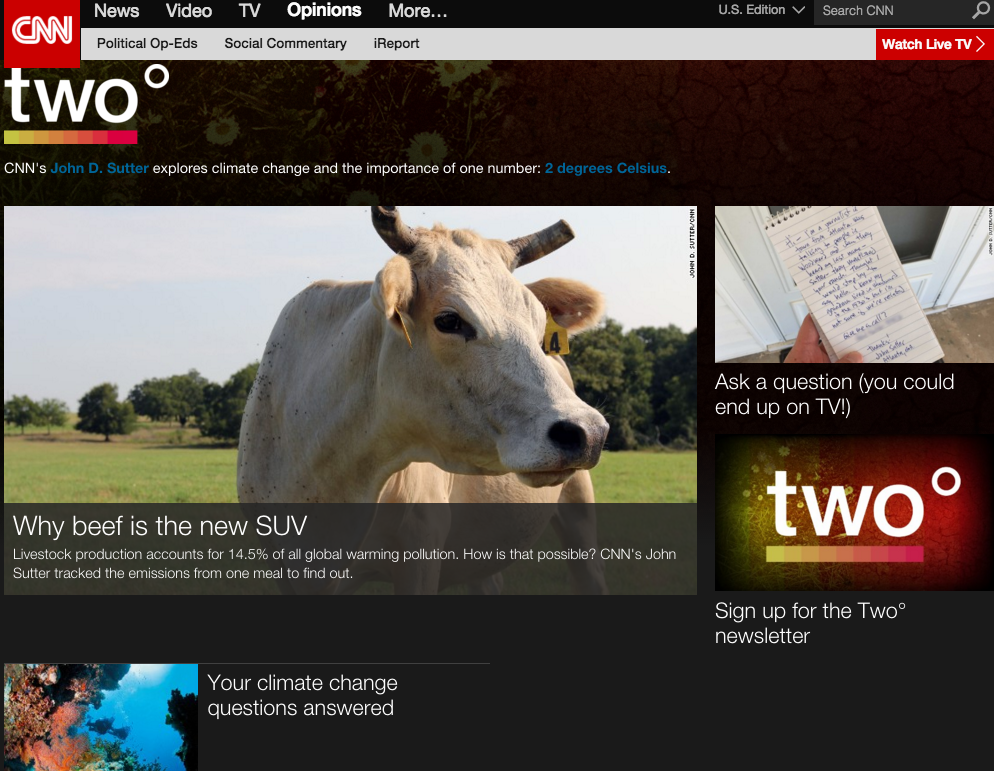
\includegraphics{graphics/CNN.png}
\end{figure}

CNN Digital columnist John D. Sutter shepherded two major crowdsourcing projects in the last couple of years, and the audience input he collected prompted the American Society of News Editors to award him the 2015 Batten Medal.

In June 2013 he launched CNN's \href{http://www.cnn.com/specials/opinion/change-the-list}{Change the List} project, asking people to bring change to the ``bottom of the list.''%\autocite{CNN}
 He invited people to pick five stories from a list of 20 they wanted him to tackle. Seven days and 32,546 votes later, he had his tally. On top was a story about America's widening rich-poor gap, which got 16,789 votes---nearly half the total.

``At the time, that really surprised me in terms of stories people would be clamoring to read about,'' he said.%\autocite{CNN}
 However, as his reporting progressed, he added, ``I really saw how central that is to what's going on in this country.''

The other \href{http://www.cnn.com/2013/06/18/opinion/sutter-ctl-vote-results/}{top-voted topics} also surprised him.\autocite{column} They paved the way for stories about the poor kids of Silicon Valley, the world's most-trafficked mammal (the pangolin), why Alaska is the national epicenter for rape, and America's most endangered river (California's San Joaquin). Plus, he generated a list of \href{http://www.cnn.com/2013/06/14/opinion/sutter-ctl-97-ideas/index.html?hpt=hp_c4}{97 other suggested topics}.\autocite{column} 

Sutter confessed that only 9 percent of the voters wanted to read about the country with 100,000 new cases of leprosy per year, which would have been his ``top pick.''

``This is journalism as democracy---rebalanced to give you power,'' he told contributors in a \href{http://www.cnn.com/2013/06/18/opinion/sutter-ctl-vote-results/index.html}{column}.\autocite{column} Sutter said his aim is to get readers more invested in stories they might otherwise ignore, such as certain social justice issues.  

He also acknowledged that the feedback wasn't all positive. Some 
``have tweeted me that this is ‘not journalism' because the story-selection is crowdsourced. Others called it a gimmick or a marketing ploy,'' he wrote.\autocite{column} Still others thought they should have been asked to submit whatever story ideas they wanted, rather than voting from a list. 

Either way, Sutter said in an interview, ``I think there was real wisdom in the crowd.''%\autocite{CNN}

In mid-August 2015, he launched a new crowdsourcing project, \href{http://www.cnn.com/specials/opinions/two-degrees}{Two Degrees}. It focuses on ``the most important number you've never heard of.'' Namely, how to avoid a global temperature rise of 2 degrees Celsius, which is regarded as the threshold for ``dangerous'' climate change.%\autocite{CNN}
 The project was an intended lead-up to climate talks in Paris at the end of 2015. 

First, Sutter asked which climate ``villains'' he should write about---voters could pick from four suggestions. The winner, again to his surprise, was animal agriculture (3,942 votes). ``I was surprised people knew about it and wanted to hear about it,'' he said. ``People are concerned about greenhouse gas emissions, with eating meat especially,'' he said. Globally, he noted, livestock contribute only about 14.5 percent of all these emissions.

Sutter does most of his call-outs on Facebook, Twitter, and in his columns. He's learned to shorten the time frame between when people first vote on the topics and when the stories actually appear. This allows people to realize they had a stake in making them happen. And he notes that CNN has invested a lot of resources in his reporting. He has traveled to Southeast Asia, Alaska, the Marshall Islands, and Silicon Valley. 

For Sutter, crowdsourcing these story lists has been “central” to his CNN work for the last couple of years. ``We don't know everything that's important in the world,'' he said. ``We need to do a better job of listening'' to citizens.

Plus, he said, ``It's taken me to topics I would not have done.''

\section{ Witnessing}  

News organizations find it highly useful to seek out information and images from people who have personally witnessed breaking news situations. However, they're also increasingly plucking these call-outs for eyewitness contributions from social media channels.  

Examples include shared images and information from the Nepal earthquake, Hurricane Katrina, the Fukushima nuclear accident, Superstorm Sandy, Andy Carvin's Twitter coverage of the Arab Spring,\autocite{Carvin} and WNYC's \href{http://www.wnyc.org/story/105465-2-mapping-storm-clean/}{crowdsourced photos} of shoveled show during the 2010 New York City blizzard.\autocite{Storm}

At the \href{http://www.watershedpost.com/}{Watershed Post}, a digital-first news website in New York's Catskills region, co-founders Julia Reischel and Lissa Harris made national news in 2011 when Hurricane Irene barreled through, flooding entire villages, washing out highways and bridges, and cutting off communications. ``The only way to keep an eye on our coverage area was to have a distributed network of people feeding us information,'' Harris said, adding that official sources were largely absent on the communications front.%\autocite{ReischelHarris}

Similarly, as Hurricane Irene was zeroing in on New Jersey, urban planner Justin Auciello launched \href{https://www.facebook.com/JerseyShoreHurricaneNews}{Jersey Shore Hurricane News}, a Facebook page that crowdsourced information not only to produce news, but also to come to the aid of local communities.%\autocite{JSHN}
With user input, Auciello reported who needed help, where people could get water or generators, where they could find their lost dogs, and how they could find family members. The page went from 20,000 likes in its first four days to 65,000 some 14 months later, October 2012, on the eve of Superstorm Sandy. JSHN now has 225,000 Facebook likes and more than 10,000 Twitter followers.%\autocite{JSHN}

Eyewitness crowdsourcing is also taking root in the area of citizen-science journalism. In 2011, when climate journalist Julia Kumari Drapkin found herself struggling to connect esoteric scientific results with on-the-ground topics that could engage local communities, crowdsourcing emerged as a way to bridge the gap. ``It's difficult to scale down from global time and space to any individual person's story or local community's experiences,'' Drapkin said. ``It wasn't like I wanted to be a crowdsourcer. It was more like, ‘This is a problem that I think the crowd could help solve.'''%\autocite{Drapkin}

She did this through her Colorado-based KVNF public radio venture \href{https://www.iseechange.org/}{iSeeChange}.\autocite{iSeeChange} Drapkin collected local observations and solicited community questions about environmental changes people were seeing, then brought in scientists to answer those questions. Some of these conversations foreshadowed large-scale natural events. For instance, when a local fire department official shared observations about fire season beginning earlier and lasting longer, scientists and researchers corroborated the official's insights, which he shared three months before the epic 2012 Colorado wildfire season.

``A lot of science disregards the anecdote,'' Drapkin said. ``However, when you've lived in the same place for your whole life and you can say, ‘Hey, I've never see this before,' more often than not those moments are opportunities to bring data to researchers and wonder if it isn't something to pay attention to.'' 

\section{ Sharing Personal Experiences}
 
Several news organizations have developed a suite of stories by issuing both structured and unstructured call-outs to targeted communities. While they might maintain a general outline of the stories they want to do, they seek contributions that may change the narrative, reveal surprising trends, uncover unknown sub-groups, or point to discrete stories for coverage. 

Honolulu's \href{http://www.civilbeat.com/projects/living-hawaii/}{Civil Beat}, for instance, crowdsourced part of its “Living Hawaii” series, publishing \href{http://www.civilbeat.com/projects/living-hawaii/%5D}{first-person narratives} from residents. ``Nothing is more common in Hawaii than struggling with the cost of living,'' said deputy editor Eric Pape. ``It's so damn expensive here. This allows people to say, `Here's my story about this.''' %\autocite{Pape}

Civil Beat also invited first-person narratives and opinion about the conflict over Mauna Kea, a dormant volcano where scientists are looking to build a telescope on what many residents consider sacred land. Pape said the topic reflects the differences of opinion in Hawaii about a number of issues: how people think about native Hawaiians, money, nature, science, etc. “It's a sweet spot for us,” Pape said. ``We are here to highlight problems and obstacles to solutions, as well as possible solutions.'' %\autocite{Pape}

Sometimes these crowdsourcing efforts begin such robust conversations that news organizations take an additional step and create venues such as Facebook pages for continued discussions after the stories are produced.

During Elizabeth Rosenthal's work on health care costs, \textit{The New York Times} eventually permitted a Facebook Group page that now has more than 6,500 members. Rosenthal acknowledges that it's an open page where any journalist can lurk and mine story ideas just as she does. ``I think my editors feel that's fine. But that was a discussion,'' she said.%\autocite{Rosenthal}

Similarly, \href{https://www.facebook.com/groups/patientharm}{Pro Publica's Patient Safety Facebook Group} of more than 3,300 members\autocite{Group} grew out of \href{https://www.propublica.org/series/patient-safety}{reporting} by Marshall Allen, Sisi Wei, and Olga Pierce that found one million people each year suffer harm when treated in the U.S. health care system.\autocite{Safety} They explored everything from dangerous dialysis centers, to unsafe hospitals, to surgical complications in operating rooms. 

Overall, ProPublica has been a leader in eliciting personal contributions that help structure new narratives.

\subsection{Case Study---ProPublica}

\begin{figure}
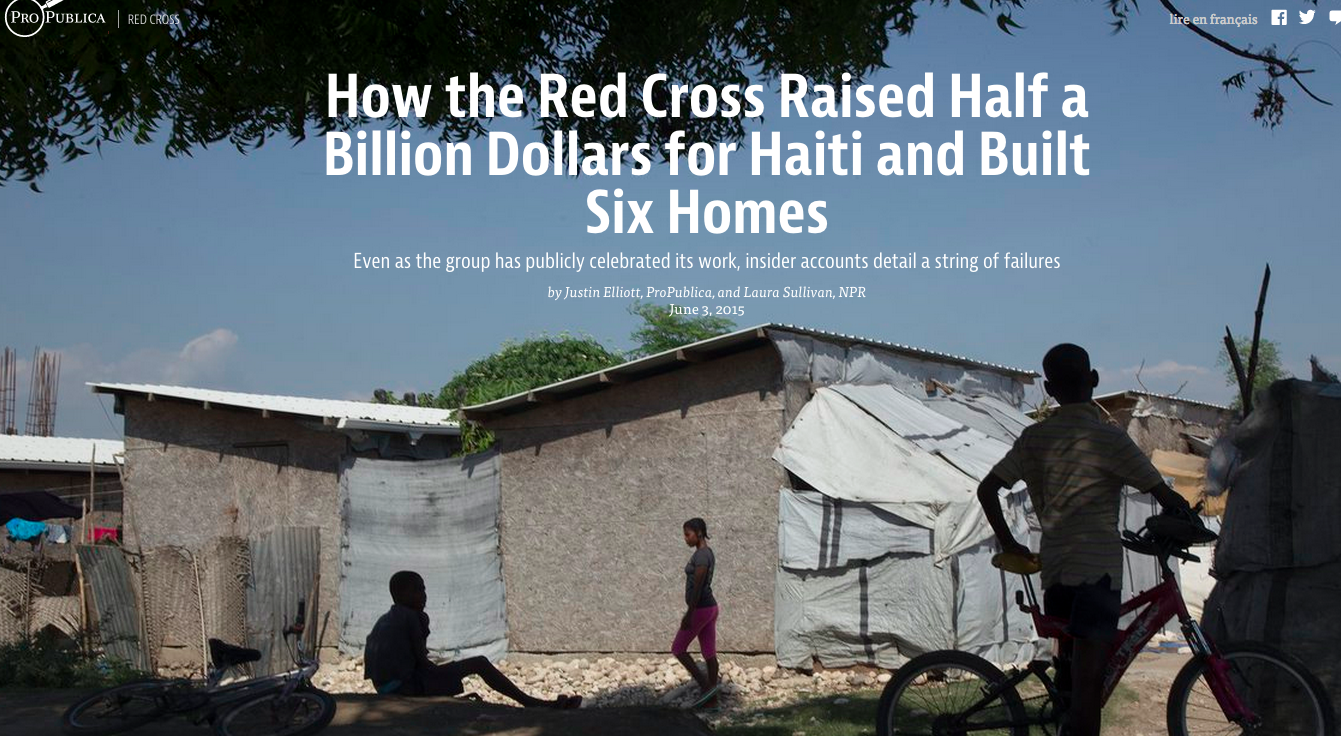
\includegraphics{graphics/RedCross.png}
\end{figure}
 
No other U.S. news organization has cultivated the art of crowdsourcing like ProPublica. With patience and acumen, the eight-year-old nonprofit startup has both embraced a unique mindset and developed a robust toolkit to transform enterprise journalism.

The mission, simply put, is to ``find people in the know,'' said Amanda Zamora, senior engagement editor who has spearheaded ProPublica's crowdsourcing efforts in recent years. That is accomplished by building ``getting involved'' on-ramps, and soliciting sources and contributions through formal call-outs. It also entails cultivating source communities with high-touch communication and dynamic givebacks.

``It's sort of like we're building a tree. We plant one and it's very skinny, but we soon get a sense of whether it's about to grow,'' she said.%\autocite{Zamora}

ProPublica's mindset is all about transparency and collaboration. ``One thing ProPublica is not afraid to do is to investigate in the open,'' said Charles Ornstein, who credits crowdsourced contributions for advancing many of his health care stories, including Dollars for Docs and experiences with the Affordable Care Act. ``You sort of announce what you are working on. It's sort of scary letting other people know. But you are also staking your turf.''%\autocite{Ornstein}

Last year, ProPublica moved away from Google Forms because it needed to better organize the vast amounts of data it was gathering. As of mid-September 2015, Zamora counted at least 37 call-outs since 2009 that generated 10,953 responses just from surveys. Another 13,400 people have signed up to participate in other ways.

ProPublica found a solution in Screendoor, a database tool built to handle government requests for proposals. ``We've taken their RFP platform and turned it into a story platform,'' Zamora said.

Over the years, crowdsourcing has contributed to an array of ProPublica news exclusives focusing on patient safety, nursing home inspections, its Surgeon Scorecard, and more. Input comes via call-outs and questionnaires and also through its ``Reporting Network'' of volunteers who engage in reporting tasks such as reviewing political ad spending in its Free the Files project.\autocite{Files}

ProPublica deploys both structured and unstructured solicitations to collect personal stories and documents, identify sub-groups with stories to tell, and build communities of stakeholders.  

Here's how one recent structured call-out worked. In late June 2015, Charles Ornstein and \textit{The Virginian-Pilot}'s Mike Hixenbaugh wanted to explore the effects of Agent Orange on Vietnam veterans and their children. They also wanted insights on stories they didn't know about.

So, ProPublica invited service members and their families to share their experiences. Ornstein wrote an advance story, then ProPublica went to work issuing call-outs for information on its website, in social media channels, and in a podcast. It also mined veterans' communities---even the websites of naval ships dispatched to the war zone. 

In the first 12 weeks, more than 2,900 people responded. ``This is an extraordinary response,'' Ornstein said. ``People want to share their stories. They've been waiting for this opportunity.''

Screendoor captured their stories in its highly searchable database. Terry Parris Jr., ProPublica's community editor, began to solicit documents to verify dates of service, wrangle photos, and record audio stories. ``I'm on the frontlines of the community coming in,'' he said.%\autocite{Parris}

By mid-September, the crowdsourcing helped generate an early story on a subset of stakeholders: the Blue Water Vets, who were being denied benefits because they sailed not in the brown waters of Vietnam's inland waterways but in the blue waters of the seas off Vietnam, where they likely drank Agent Orange-polluted water.

Not all of ProPublica's crowdsourcing efforts involve requests to complete questionnaires. In fact, significant stories by Justin Elliott, Jesse Eisenberg, and NPR's Laura Sullivan on Red Cross relief spending during the 2012 Superstorm Sandy and the 2010 Haiti earthquake initially engaged in an unstructured call-out. Essentially, the journalists urged readers to email Justin ``if you have experiences with or information about the Red Cross, including its operation after Sandy.''

Only a few emails arrived at first, until ProPublica reported that the Red Cross was fighting its FOIA request to the N.Y. Attorney General because the information might potentially disclose ``trade secrets.'' More sources weighed in, leaked documents arrived, and people urged the reporters to look into Haiti relief spending as well.  

``There's no way we would have gotten the tips we got without that [email us] line,'' Elliot said. ``People need a nudge. Just because of Sandy, I've been adding these lines to everything I've written.''

The ProPublica/NPR reports raised questions about how the Red Cross spent millions in donations raised for victims. One impact: recently proposed federal legislation requiring the charity, which has a government-mandated disaster-response role, to open its operations to outside oversight.

``Universally, these are people who worked for or volunteered for the Red Cross for a long time,'' Elliott said. ``They cared a lot about the organization and thought there were unethical decisions . . . might be some management incompetence or mismanagement of money.''  

Said Zamora, ``Every reporter who has worked on a call-out will tell you they found sources or insights that substantively impacted their stories.''

One outcome of ProPublica's crowdsourcing is ``we have way more stories and sources than we can use,'' said Zamora, who wants to ``catalyze other reporting'' by making that data available to journalists who want to find their own stories in it.

Screendoor will play a role in managing that network of reporters because it can identify contributors by location. The database, said co-founder Clay Johnson, sends an immediate acknowledgement to a contributor. It allows ProPublica to filter and rate responses, add comments into the responses, send a note to a specific sub-group of people, track the emails sent, and share all project updates with participants in a personalized way. 

``I can say, ‘Dear Barry,''' Ornstein said. ``You told us you have cancer, diabetes, or [suffered from] a heart attack.''

Zamora also plans to use it to ``dynamically expose pieces of the story'' through vignettes, pull quotes, or audio clips from contributors so ProPublica can continue giving back to the community and tease out more input while the crowdsourcing process is ongoing.%\autocite{Zamora}

Next up: ProPublica is partnering with Yelp in a project to align Yelp's ``qualitative reviews with ProPublica's objective data'' on medical services, Ornstein said. He added that the partnership will give ProPublica access to Yelp's ``firehose'' of more than a million reviews.%\autocite{Ornstein}

The Knight Foundation recently awarded ProPublica a \$2.2-million grant to help advance its audience engagement work and train others in its techniques. ``I feel we are just on the cusp of finally being able to realize what I've wanted to do,'' Zamora said.


\section{ Tapping Specialized Expertise}

In some instances, journalists recognize that they have gaps in knowledge that are hard to fill with standard reporting techniques. Sometimes that's because data may be buried in privacy policies or trade-secret lockboxes. 

As ProPublica developed its ``Patient Safety'' series, it particularly tapped a sub-group of health care providers to help it develop its \href{https://projects.propublica.org/surgeons/}{Surgeon Scorecard}.\autocite{scorecard} The scorecard calculated death and complication rates for surgeons performing one of eight elective procedures under Medicare.

Several public broadcasters have been in the vanguard of using crowdsourcing to gather health care data from individual consumers. Most recently, KQED in San Francisco, KPCC in Los Angeles, and WHYY in Philadelphia asked hundreds of listeners to share specific prices they paid for certain medical procedures. The results helped others in those cities compare prices that different providers charged.%\autocite{CHC}
(Read more on the \href{http://towcenter.org/crowdsourcing-in-theory-and-practice}{Tow Center's blog} about the newsrooms' partnerships with ClearHealthCosts.com, which was founded by Jeanne Pinder, a co-author of this report.%\autocite{Towblog}
)

When the International Consortium of Investigative Journalists (ICIJ) landed massive troves of leaked documents that were too big for one news organization to analyze alone, they tapped members around the world to leverage their knowledge of local individuals and entities whose names appeared in the data. ``Maybe we would call it a more structured kind of crowdsourcing,” said ICIJ deputy director Marina Walker Guevara. “We take steps to carefully select our crowd.''%\autocite{ICIJ}

ICIJ's first big disclosure, \href{http://www.icij.org/offshore}{Offshore Leaks}, published in April 2013, involved 100 journalists from 60 countries examining 2.5 million records of some 130,000 offshore accounts, according to a case study of the initiative.\autocite{Buzenberg} The stories made transparent who owned covert companies and private trusts, often used to dodge taxes. ICIJ later put some of the information in a \href{http://www.icij.org/offshore/search-offshore-leaks-data}{public database}, subsequently used by more than 400 reporters to develop their own stories.%\autocite{ICIJ} 
 ICIJ went on to develop two more initiatives---Lux Leaks and Swiss Leaks---with selective crowdsourcing from scores of journalists.\autocite{Buzenberg} 


\section{Completing a Task}

At times, news organizations need help performing specific journalism jobs that they don't have the resources to do themselves, so they issue call-outs to volunteers. ProPublica, for instance, tasked citizens with poring over records of campaign advertising in its notable Free the Files project, and it asked for volunteers to call all 535 members of Congress to help report who was getting free \href{http://www.propublica.org/getinvolved/item/propublicas-super-bowl-blitz-which-congressmen-are-getting-super-bowl-perks}{Superbowl perks}.\autocite{perks}

D. Brian Burghart built his \href{http://www.fatalencounters.org}{FatalEncounters.org} database with more than 8,800 cases of ``people killed during interactions with law enforcement'' by calling for volunteers to submit incidents and verifying those and others with web research and public records requests.%\autocite{Burghart}

Australia's ABC runs ABC Open,\autocite{ABCOpen} an example of a traditional news organization thinking creatively about using crowdsourced methods to reach previously untapped communities. ABC Open is a participatory media project that sends over 45 producers out to hold digital-skills workshops for rural Australians. The intent of the initiative is to provide Australians outside metro areas with an opportunity to tell stories. ABC Open encourages them to contribute stories to its website with periodic story prompts. Since 2010, about 12,000 people have shared some 80,000 submissions. 

In ABC's news division, an interactive team led by Matt Liddy collected a year's worth of a metadata from the phone of an ABC reporter and tasked its audience with uncovering insights by exploring the data.%\autocite{Liddy}
 The high-bar effort, intended to show audience members how phone metadata can tell stories, resulted in over 400 people sifting through the data themselves and writing to ABC News with their findings.\autocite{ABCNews}

Still, the journalistic leader in tasking volunteers with crowdsourced requests has been \textit{The Guardian}. Since 2009, it has tapped into the power of its audience base, expertly finding ways to work collaboratively with its large and active audience. As time has passed, \textit{The Guardian} has learned how to target specific communities with clear asks, while simultaneously broadening the types of answers it is open to receiving. The result is a seamless, back-and-forth interaction that benefits all parties. 

\subsection{Case Study---\textit{The Guardian}}

In 2009, \textit{The Guardian} established itself as a frontrunner in crowdsourced journalism with its famous MPs' expenses experiment: the organization created a searchable database of thousands of MPs' spending receipts and asked the public to help mine the dataset for interesting information.

The experiment was a resounding success. Over 20,000 volunteers searched more than 170,000 documents, setting a new standard for the potential of crowdsourced journalism to produce high audience engagement and tangible journalistic outcomes. 

In the six years since, crowdsourcing has become an integral part of \textit{The Guardian}'s strategy, said Oliver Laughland, senior reporter at \textit{The Guardian U.S.}%\autocite{Laughland}
 ``The journalists who work here have [crowdsourcing] ingrained in their consciousness. We're always trying to think about ways in which you can engage with the audience and make them part of it.''

\textit{The Guardian}'s latest effort, The Counted, exemplifies this.\autocite{Counted} The Counted is an attempt to track the number of people killed by police and law enforcement agencies in the United States. It aims to provide a database that is currently at the center of national attention due to recent high-profile citizen deaths at the hands of police and security officers.

For \href{http://www.theguardian.com/us-news/series/counted-us-police-killings}{The Counted}, Laughland said the role of the audience was even more crucial than usual. ``We knew The Counted wouldn't work without it.''%\autocite{Laughland}

The Counted lives at the intersection of crowdsourced data collection and traditional reporting methods. In many cases, the team starts with data reported by members of the community, then gives that data to reporters to verify and extend. Occasionally the situation is reversed: a journalist will call up local police departments or medical examiners to create a data point that is updated as more information comes in from the crowd. 

The result is that The Counted includes a number of stories that are outside the reach of both smaller and larger news organizations, and the campaign has the resources to report on stories that otherwise would have fallen through the cracks. ``From a traditional reporting perspective, you can report on cases that haven't captured national attention before,'' Laughland said, citing five or six deaths that had not yet been reported. 

Mary Hamilton, audience editor at \textit{The Guardian U.S.}, said these stories are told primarily by reaching out to specific, interested communities rather than the organization's general audience.%\autocite{Hamilton}
 As a result, journalists' existing ties to community networks were instrumental for initially spreading the word.

The team also has a distributed email list with semi-regular updates, and a project Facebook page and Twitter account that share news on police killings and make appeals for information on specific cases. All of these accounts feed into the \href{http://www.theguardian.com/us-news/ng-interactive/2015/jun/01/the-counted-police-killings-us-database}{interactive},\autocite{MPExpense} where the team has been meticulous about the tone and language they use. ``Join our community'' is the phrase they've adopted precisely for its emphasis on inclusion and action. 

Keeping momentum going during a year-long effort is daunting, but Hamilton credits two factors for the team's ability to continually engage its audience: regularly adding new content (in the form of updates to the email list, Facebook page, Twitter account, and online interactive) and an element of reward. 

Every single tip the team receives is viewed, counted as significant, and responded to, Hamilton said. ``You can't have a meaningful, long-lasting crowdsourced project without this type of acknowledgement.''

The Counted was also designed to support multiple entry points through which community members can engage and submit information.
Hamilton noted that different mediums yield different types of information. On Twitter, the team is more likely to receive links. The Facebook page generates a mix of submissions: community members have more space to talk about leads they might have or to engage in conversation with other world-be contributors.

Hamilton said the most meaningful information often comes from the Tips Form on \textit{The Guardian}'s website. It is here that family members or members of the deceased's legal team will provide fleshed-out stories and accounts. Submissions through the Tips Form have been so well detailed that they have led, on occasion, to published Op-Eds on \textit{The Guardian}'s main site.

Users usually travel across the different platforms before eventually settling on one. ``They tend to gravitate to whatever they're most comfortable with,'' Hamilton said.

As of September 2015, The Counted has reported over 837 people killed by U.S. law enforcement agencies, with many of those cases reported entirely because of the project's crowdsourced element. As Hamilton said, ``Our readers collectively can scour far more than we can. They're fantastic at holding us to account and making sure that our reporting is accurate.'' 

But there are costs. ``This takes resources,'' she noted: 
\begin{quote}
This is a significant amount of work for my team . . . It's at least two hours a day every day, including weekends---all the moderating, going through submissions, responding. The journalism has to be updated, has to continue to live after the launch point. The community engagement part is work, just as much as writing the story in response to the community engagement is. Resourcing that carefully is hugely important, and that work is often invisible. \end{quote}

One of the major takeaways is that successful crowdsourcing demands work, time, and effort. ``Crowdsourcing and engagement aren't an afterthought,'' Hamilton said. ``You don't build the journalism and then decide how you're going to do an engagement effort. You have to plan it from the start. It's not the icing. It has to be baked in.'' 

\section{Engaging Audiences} 

Not all crowdsourcing is intended to produce investigative series, build sophisticated databases, or tease out powerful narratives from people with knowledge of something reporters want to pursue.

Many news organizations are making it a priority to connect with their audiences in ways that are as much fun and engaging as they are informative. Others connect with real-time, useful information.  

``Whenever we have active weather, crowdsourcing is at the heart of what we do,'' said Jason Samenow, \textit{The Washington Post}'s weather editor. He is also chief meteorologist for the Post's Capital Weather Gang, marshaling contributions from its 180,000 \href{https://twitter.com/capitalweather?ref_src=twsrc%5Egoogle%7Ctwcamp%5Eserp%7Ctwgr%5Eauthor}{Twitter followers} and 66,600 Facebook fans. During snowfalls, ``people send us pictures of their rulers in the ground,'' he said.%\autocite{weather}

Likewise, the for-profit NYC's CleverCommute.com is now transitioning hundreds of thousands of email contributors to a new app that will collect their alerts on real-time commuter train hiccups and relay them to New York's huge commuter train community and local media clients.%\autocite{Commute}

Public broadcaster WNYC is one of the standouts in crowdsourcing its listeners about everything from the useful (e.g., has the city snow-plowed your street yet?) to the whimsical (e.g., what is your sleep pattern?).
``We need to be good at this because it's the source of very valuable content,'' said Jim Schachter, WNYC's vice president for news.%\autocite{Schachter}

Public radio, with its well-received call-in shows, is uniquely situated to develop call-outs that command a lot of contributions, as well as donors. ``In Bored and Brilliant, we asked you to build a replica of your dream house out of the contents of your wallet and then take a picture of it and share it with us,'' Schachter said. ``If you're willing to do all that work, it's a fairly small ask of us to say, ‘Will you be a member?'''


\subsection{Case Study---WNYC Public Radio}

WNYC public radio in New York specializes in crowdsourcing with intense community engagement. Recent projects have tasked listeners with tracking soil temperatures to predict when cicadas would emerge from the ground, to assessing their sleep patterns and encouraging them to turn off their mobile phones and test their creativity in its Bored and Brilliant challenge.

What's the secret? ``It has to do with purposefulness and a reasonably active effort to learn from what we've done in the past,'' said Jim Schachter, WNYC's vice president for news. ``When we launched into the sleep project, we were thinking what worked and didn't work in the cicada project. And when we launched Bored and Brilliant, we were thinking what worked and didn't work in sleep and cicada.''

Part of the station's secret sauce? Its popular Brian Lehrer morning call-in show. 

``We have a call-in show and host that for 25 years have been honing how to pose questions to people so the board will light up and Brian won't be there talking to himself,'' Schachter said. ``I don't want everybody else to start a talk show because our secret weapon would be stolen. But if every newsroom acted like it had one, what would it be like for that newsroom?''

Integral to many projects is John Keefe, senior editor for data news. A journalist with technical skills, Keefe was central to the \href{http://project.wnyc.org/cicadas/}{Cicada Tracker project}, which provided directions on how to build a soil-temperature measuring device.\autocite{Cicadas} Ultimately, 1,500 temperature readings came in, many from people who built the tracker themselves.%\autocite{Keefe}

In the 2014 project \href{http://www.wnyc.org/story/clock-your-sleep-findings/}{Clock Your Sleep}\autocite{Sleep} almost 5,000 people signed up to log sleep patterns for several weeks, either online, with a Fitbit or other device, or by using WNYC's iPhone app built for the project. 

The project had multiple on-air appearances because, Keefe said, ``For a longer study, you need a reminder.''

\href{http://www.wnyc.org/series/bored-and-brilliant/}{Bored and Brilliant}\autocite{Bored} enticed people with a week of challenges to put away their cell phones and ``take part in a semi-scientific experiment to test your creativity.'' The project nudged people to reclaim the time they spend on their phones and use it instead to let their minds wander ``and see what brilliance it may lead you to.” One challenge, a photo-free day, urged people to `see the world through your eyes, not your screen.'''

\begin{figure}
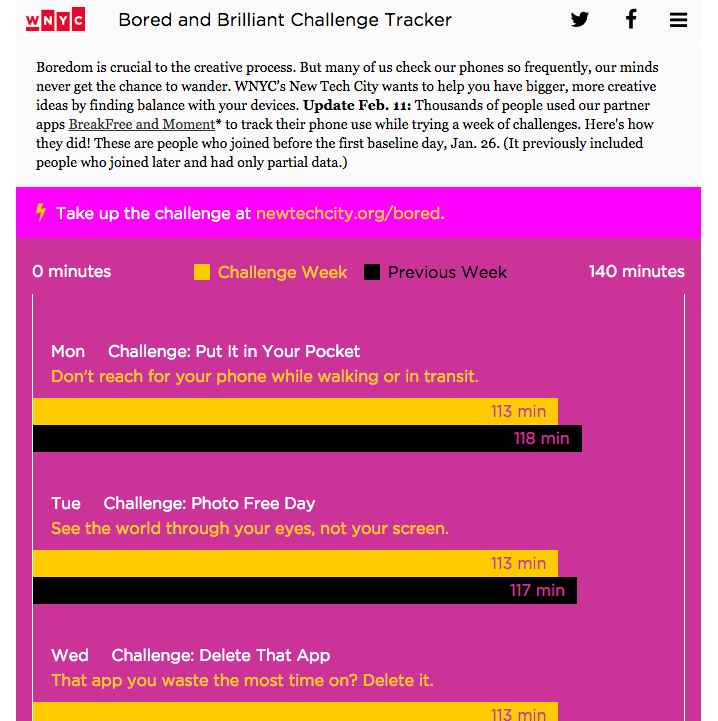
\includegraphics{graphics/CrowdsourcingWNYCBredAndBrilliant.png}
\end{figure}

``It was an activity you could do yourself and it made you think about the topic,'' Keefe said. More than 20,000 people took part.

While much of WNYC's work focuses on engagement rather than investigations, hard news also plays a role. In \href{http://www.wnyc.org/story/105548-2-mapping-storm-clean-/}{Mapping the Storm Cleanup}, WNYC sought to truth-check Mayor Michael Bloomberg's assertion that snow-shoveling had been effective city-wide after a 2010 blizzard.\autocite{Storm} 

WNYC invited listeners to text if their streets had been plowed. ``We could map the no's vs. the yeses. And since we had their phone numbers, we could text them back the next day, or two days later, and say, ‘Is your street plowed now?''' Keefe said. The result: a series of maps with pins, white for unplowed and blue for plowed. Over three days of mapping, the pins turned from white to blue. 

``It's easy to get people to participate if they're angry,'' Keefe said. ``It's harder . . . if it's benign.''

In September 2010, when New York City shifted from using voting machines to paper ballots that were marked by a voter and then scanned into a machine, WNYC launched \href{http://www.wnyc.org/story/94305-text-ballot-your-primary-day-reports/}{Your New Ballot Stories}, expecting ballot 
design to be a big issue.\autocite{Ballot} 

The station asked people to sign up before the vote so it could text them on voting day and, if they voted, invite them to tell what happened, or to leave a voice message that could be used on the air. 

As it turned out, ballot design was not the biggest issue. Instead, voters expressed concerns about ballot privacy after being asked to hand their ballots to poll workers for scanning. ``The privacy issue popped up, and that was our story right away,'' Keefe said.

Accuracy is sometimes an issue, Keefe noted, and WNYC has certainly rejected some projects because they are not accurate enough. After Hurricane Sandy, he said, WNYC thought about crowdsourcing which gas stations had gas, but didn't: first, because it couldn't ensure the information would be accurate, and second, because people might use their last gas to get to a station, only to be disappointed. ``It's too fragile a situation to crowdsource,'' he said. 

That journalistic sensibility, infused with humility, lies at the heart of WNYC's crowdsourcing.

``That's what it's about,'' Schachter said. ``It's a genuine expression of humility that the audience, however you're defining it for a particular endeavor, knows more than you do---and it's to be listened to. That's really important.''

\chapter{Verification and Legal Issues}

Many news outlets say they're not comfortable trusting information that arrives via crowdsourcing. But those who are deeply engaged in the process say accuracy is seldom a problem. Newsrooms will undertake verification as needed. When ProPublica, for instance, uses an Agent Orange story from a Vietnam veteran, it takes care to ask for records documenting military service. But when WNYC asks about your sleep patterns, verification is not necessary.

Crowdsourcing does open doors to some legal issues. In building a crowdsourcing project, it's important for a news organization to establish terms and communicate how community contributions will be used. 

``When you're soliciting information, you get to set the terms,'' said Jennifer Dukarski, a media attorney at Butzel Long's Ann Arbor, Michigan, office. ``When they send stuff back to you, you can use it in any way that you told them you're going to use it.''%\autocite{Dukarski}
 Most crowdsourcing practitioners advise being clear about your plans for the stories and data you collect.

Likewise, if a news outlet is capturing and using pictures or videos from Twitter, Facebook, Instagram, or another social media platform, the journalists must observe that platform's terms and conditions regarding intellectual property. ``Usually the people who created it will retain the rights and copyrights,'' Dukarski said. (\href{http://eyewitnessmediahub.com/%5D}{Eyewitness Media Hub} is one new resource for best practices and sourcing, verifying, and obtaining rights to materials.)%\autocite{EyewitnessMediaHub}

Journalists may also wonder if they have legal liability if a crowdsourcing contributor lies, defames, or libels someone. ``As long as you're not encouraging it or doing it yourself, but only acting in the capacity of providing space for people to express their views, you're protected by the Communications Decency Act,'' Dukarski said. Section 320 of that act gave web services broad immunity from liability for content posted by users. 

Most often, however, journalists use crowdsourcing contributions as elements in reporting a story and not as discrete pieces of content populating a publishing platform.

Moderating or editing comments can be an area of concern. ``When someone sends in a comment, if you start modifying and create defamation, then you own the defamation,'' she said.

Dukarski also added that crowdsourcing can raise privacy issues. She recommends that media organizations ``continue to be diligent and sensitive'' about identifying people's addresses, home phone numbers, and other personal information. 


\chapter{Lessons Learned} 

Contrary to popular belief, the respondents who devote the most time to crowdsourced campaigns are often those who have the highest level of expertise in the subject, said USC professor Daren Brabham, who has researched online crowdsourcing. 

``It's a better use of your time to target people who are experts and already interested in the topic, and then work from there,'' Brabham said. ``Once you get a hardcore community involved, others will be intrigued by the excitement, and it will bubble up from there.''\autocite{BrabhamAmateur}

ProPublica's Zamora observed that sources from ``closed-rank'' communities, such as health care providers, tend to generate fewer contributions than from patient communities. Also, when ClearHealthCosts and its California PriceCheck partners asked about IUD prices in San Francisco and Los Angeles, the response was limited. The community was more interested in colonoscopy prices, a likely testament to public radio demographics.%\autocite{Aliferis}

\chapter{Conclusion} 

Our research shows that crowdsourcing has been credited with helping to create amazing acts of journalism. It has transformed newsgathering by opening up unprecedented opportunities for attracting sources with new voices and information, allowed news organizations to unlock stories that otherwise might not have surfaced, and created opportunities for them to experiment with the possibilities of engagement just for the fun of it.

In short, it has done just what the pundits predicted a decade ago: helped turn journalism into more of a conversation than a one-way megaphone. 

Crowdsourcing is also credited with shaping journalism into more of an iterative process: as data or stories come in from contributors, reporters see new possibilities for their journalism---and news organizations see opportunities to incrementally publish those contributions in ways that tease out more. 

Moreover, once communities of sources are built, they can be retained forever---if news organizations take care to maintain them with updates and ongoing conversation.

But crowdsourcing can be high-touch and high-energy, and not all projects work the first time. 

For all its potential, crowdsourcing's promise is widespread and systemic at just a few big news organizations---ProPublica, WNYC, and \textit{The Guardian}, for example. At other mainstream news organizations, like CNN Digital and \textit{The New York Times}, only a handful of reporters and editors---and not the institutions themselves---are the standard bearers. 

To be sure, crowdsourcing businesses are flourishing outside of journalism. But within the news industry, wider systemic adoption may await more than enthusiasm from experienced practitioners and accolades from sources who welcome contact.  

We would like to see more research and evidence exploring whether crowdsourcing can foster increased support for journalism. That support might take the form of audience engagement, such as attention, loyalty, time spent on a site, repeat visits, or contributing personal stories. Or it might involve financial support from members or donors, from advertisers who want to be associated with the practice, or from funders who want to support it. 

Also to be explored is whether crowdsourced stories have more real-world impact, such as prompting legislative change, than other types of journalism do. 

Until this data is available and a better suite of tools and practices is developed, some news organizations may be wary of joining the ranks of long-time practitioners and investing the time and resources needed to support crowdsourcing projects.

However, newsrooms that do support crowdsourcing are pushing it in new and interesting directions. One hallmark of this more experienced version of crowdsourcing is the idea that better crowdsourcing involves earlier integrations of community contributions, said \textit{The Guardian}'s Pilhofer. ``This is where I think crowdsourcing and journalism meet. The results can be powerful.''


\section{Best Practices in Crowdsourcing} 

The following suggestions have been drawn from our research and interviews, and from our personal experience, particularly those of ClearHealthCosts.com founder Jeanne Pinder, an author of this report. 
\begin{itemize}
\item Know your community. What motivates or frustrates them? Do they want to vent or share knowledge?

\item Identify the problem you're trying to solve. Make sure your questions elicit what you are trying to learn. But be prepared for the community to tell you if you haven't defined the problem properly.

\item Define your journalistic goals clearly. Do you want to build a database, plug gaps in knowledge, or find trends and unique stories? Are you planning a short-lived effort or a long-term series?

\item Be clear with your community about what you will do with its contributions. Will they be quoted by name in a news story? Will their information be shared for other journalists to use?

\item Define your audience engagement goals and decide how you'll measure success---clicks, shares, tweets, Facebook likes, or earned media mentions. Appearances at a state Senate committee investigating your issue can count just as much as responses to your specific question. 

\item Choose your tools carefully. You may want responses to questionnaires or data to populate a public database. Sometimes you want photos, and others you want audio or SMS responses. Network to find the best tools to match your aims.

\item User-test your tools and your call-outs inside of your work group or with a beta group of testers before going public.

\item Ask: Is this really a good crowdsourcing project? Is it something we want to turn to call-out for? Where can we mine instead of hosting a call-out?

\item Staff up and be ready for a flood of responses early on. Know, too, that some projects take a while to build. 

\item Repeat and repeat your call-outs for contributions. People may not be able to respond the first time they learn about it.

\item Pay attention to the language you use. Ask people to ``share'' rather than ``submit.''

\item Shorten the time frame between when people first vote or contribute information and when the articles actually appear so that your sources realize they have a stake in making the stories happen.  

\item Give back to your community from the start. Pre-populate a database with information. Report back to your community early and often. Email updates, use pull quotes, publish short audio stories or vignettes as part of the feedback loop. 

\item Respond to and reward your contributors. Use thank-you e-mails, on-air shout-outs, or invitations to an event. Engage with the comments. If you make an open call and walk away, your results will be diminished. 

\item Make it easy for people to contribute. Use drop-down menus with easy questions. 

\item Ask questions that steer clear of yes and no answers. Instead, tease out the stories people have to tell you. 

\item Explain to your community what they'll get. For ClearHealthCosts, the community got health care pricing data and the ability to compare their prices with others. In the WNYC sleep project, they were able to compare their sleep patterns with others'. 

\item Iterate on the fly. If something is not working, fix what you can immediately. Don't wait for the next project. 

\item Think about verification. If something seems like an outlier, check it out. 

\item Have a free-form ``notes'' or ``comments'' box and an email to capture contributions that may fall outside your questionnaire.
\end{itemize}
Above all, think of engagement as a ladder and sharing data or answering a survey as just a few of the things community members can do. They might also share a post or call-out with their own networks, tweet and comment, search the database, email, send in documents, appear on a radio show, or testify before a legislative committee. Try to capture all those things as you measure the impact of your efforts.

\section{Author Biographies}

\textbf{Mimi Onuoha, Research Fellow, Data \& Society} 

Mimi Onuoha is a formerly London-based American artist and researcher who uses data and code to explore new forms of storytelling, social critique, and interaction. Her work explores how technology and culture influence and respond to each other, as seen through datasets representing social structures and experiences.

Most recently, Onuoha was selected as part of the inaugural class of Fulbright-National Geographic Fellows, where she created \href{http://www.nationalgeographic.com/pathways}{Pathways},\autocite{Pathways} a data storytelling project derived from Londoner's mobile data. She also served as a visiting researcher at the Royal College of Art. Previously, she was a research resident at NYU, as well as a technology consultant for Brooklyn-based nonprofit Project SAFE. 

Onuoha has a master's degree from NYU's Interactive Telecommunications Program and is currently a fellow at the Data \& Society Research Institute, where she is combining ethnographic research methods with emerging data practices to investigate potential strategies for DIY and crowdsourced data collection.

Twitter: @thistimeitsmimi 
Website: \href{http://mimionuoha.com}{http://mimionuoha.com}

\textbf{Jeanne Pinder, Founder and CEO, ClearHealthCosts.com}

Jeanne Pinder is founder and CEO of \href{http://clearhealthcosts.com/}{ClearHealthCosts.com}, a New York City journalism startup bringing transparency to the health care marketplace by telling people what stuff costs. 

\href{http://clearhealthcosts.com/}{ClearHealthCosts.com} uses shoe-leather journalism, crowdsourcing, database sourcing and curation, and data visualization to reveal the mysteries of pricing. The company partners with big news organizations like \href{http://ww2.kqed.org/stateofhealth/2014/06/23/share-your-bill-make-health-costs-transparent-in-california/}{KQED public radio} in San Francisco, \href{http://www.scpr.org/price-check}{KPCC public radio} in Los Angeles, \href{http://www.newsworks.org/index.php/local/item/77899}{WHYY public radio} in Philadelphia, and MedPage Today to collect and reveal pricing information. \href{http://clearhealthcosts.com/}{ClearHealthCosts.com} has won grants from the \href{http://towknight.org/2010/12/2010awards/}{Tow-Knight Center for Entrepreneurial Journalism} at the CUNY Graduate School of Journalism, the Ford Foundation via the \href{http://www.iwmf.org/women-entrepreneurs-in-digital-news-jeanne-pinder/}{International Women's Media Foundation}, and the McCormick Foundation via \href{http://www.newmediawomen.org/site/2012_winners}{J-Lab at American University}. Current partnerships are funded by the John S. and James L. Knight Foundation and the Robert Wood Johnson Foundation.

Pinder founded the company after volunteering for a buyout from \textit{The New York Times}, where she worked for almost 25 years. At \textit{The Times}, she was an editor on the foreign desk, a reporter on the business desk, and the deputy founding editor of the Circuits technology section, as well as an editor on the metro desk and the creator of a flexible work policy for the organization. Before, she worked at \textit{The Des Moines Register}; The Associated Press; and \textit{The Grinnell Herald-Register}, her family's twice-weekly independent paper, which her grandfather purchased in 1949.

A Russian and Slavic linguistics major in college and graduate school, she taught Russian when she lived in what was then the Soviet Union. Read more about how crowdsourcing at ClearHealthCosts.com works in a \href{http://towcenter.org/crowdsourcing-in-theory-and-practice}{Tow Center blog post}.%\autocite{`Towblog'}   

Twitter: \href{https://twitter.com/chcosts}{https://twitter.com/chcosts}
Website: \href{http://clearhealthcosts.com/}{http://clearhealthcosts.com/}


\textbf{Jan Schaffer, Executive Director, J-Lab}

Jan Schaffer, executive director of J-Lab, runs one of the nation's top incubators for news entrepreneurs and innovators and is a leading thinker on the emerging new media landscape.

A Pulitzer Prize-winner for \textit{The Philadelphia Inquirer}, she left daily journalism to lead pioneering initiatives in civic journalism, interactive, and participatory journalism. She launched J-Lab in 2002 to help newsrooms use digital technologies to engage people in public issues. The center helped to fund 104 startups and pilot projects. J-Lab is the successor to the \href{http://pewcenter.org/}{Pew Center for Civic Journalism}, a \$14-million project Schaffer previously led that funded 120 pilot projects in U.S. newsrooms. 

For more than 20 years, Schaffer held a range of reporting and editing positions at \textit{The Philadelphia Inquirer}. As a federal court reporter, she helped write a series that won freedom for a man wrongly convicted of five murders. The stories led to the civil rights convictions of six Philadelphia homicide detectives and won several national journalism awards, including the Pulitzer Prize Gold Medal for Public Service. Also while covering federal courts, she broke the Philadelphia Abscam story about the FBI sting operation that used agents posing as Arab sheiks. She was sentenced to jail for six months for refusing to reveal her sources; the sentence was stayed on appeal.

Twitter: @janjlab, @jlab
Website: \href{http://www.j-lab.org }{http://www.j-lab.org} 


\section{Complete List of Interviewees} 

\begin{itemize}
\item \textbf{Lisa Aliferis}, Editor, ``State of Health'' blog, KQED (San Francisco)
\item \textbf{Olivia Allen-Price}, Interactive and Engagement Editor, KQED News
\item \textbf{Justin Auciello}, Founder, \textit{Jersey Shore Hurricane News}
\item \textbf{Greg Barber}, Director of Digital News, \textit{The Washington Post}
\item \textbf{Rebecca Blatt}, Bureau Chief, Public Insight Network, Cronkite School of Journalism at Arizona State
\item \textbf{Daren Brabham}, Assistant Professor, USC
\item \textbf{Paul Bradshaw}, journalist, Founder of Help Me Investigate
\item \textbf{Jennifer Brandel}, Founder, Hearken
\item \textbf{Carrie Brown}, Director, M.A. Social Journalism, City University of New York Graduate School of Journalism
\item \textbf{D. Brian Burghart}, Founder, FatalEncounters.org
\item \textbf{Steve Buttry}, Director of Student Media at Louisiana State University's Manship School of Mass Communication
\item \textbf{Joshua Crandall}, CEO and Founder, CleverCommute.com
\item \textbf{Jennifer Dukarski}, attorney, Butzel Long
\item \textbf{Cath Dwyer}, Co-director, ABC Open (Australia)
\item \textbf{Justin Elliott}, reporter, ProPublica
\item \textbf{Lou Ferrara}, Vice President for Sports, Business, Entertainment, News Content Verticals and Digital Products, The Associated Press
\item \textbf{Mary Hamilton}, Audience Editor, \textit{The Guardian}
\item \textbf{Lissa Harris}, Co-founder and Publisher, Watershed Post 
\item \textbf{Burt Herman}, Co-founder, Storify
\item \textbf{Amanda Hesser}, Co-founder, Food52
\item \textbf{Jeff Howe}, Program Coordinator, Media Innovation, Northeastern University
\item \textbf{Irina Ivanova}, News Editor, The Huffington Post
\item \textbf{Clay Johnson}, Founder and Chairman, Department of Better Technology (Screendoor)
\item \textbf{John Keefe}, Senior Editor for Data News, WNYC
\item \textbf{Jim Kennedy}, Senior Vice President, Strategic Planning, The Associated Press
\item \textbf{Sasha Koren}, former Deputy Editor of Interactive News, \textit{The New York Times}
\item \textbf{Julia Kumari Drapkin}, journalist, Founder of iSeeChange
\item \textbf{Oliver Laughland}, Senior Reporter, \textit{The Guardian}
\item \textbf{Matthew Leonard}, Editor, ``Upstate Insight and Innovation Trail,'' WXXI
\item \textbf{Heather Leson}, Board President, Humanitarian OpenStreetMap Team
\item \textbf{Matt Liddy}, Editor of Interactive Storytelling, ABC News (Australia)
\item \textbf{Amanda Michel}, Senior Editor of Strategy and Partnerships, \textit{The Guardian}
\item \textbf{Linda Miller}, Director, Public Insight Network
\item \textbf{Michael Morisy}, Founder, MuckRock
\item \textbf{Charles Ornstein}, Senior Reporter, ProPublica
\item \textbf{Jacopo Ottaviani}, data journalist and Project Coordinator, Generation E
\item \textbf{Eric Pape}, Deputy Editor for Innovation and Special Projects, Honolulu Civil Beat
\item \textbf{Terry Parris Jr.}, Community Editor, ProPublica
\item \textbf{Sona Patel}, Senior Social Strategy and UGC Director, \textit{The New York Times}
\item \textbf{Aron Pilhofer}, Executive Editor of Digital, \textit{The Guardian}
\item \textbf{Jeanne Pinder}, Founder, ClearHealthCosts.com
\item \textbf{Julia Reischel}, Co-founder and Editor, Watershed Post
\item \textbf{Elisabeth Rosenthal}, reporter, \textit{The New York Times}
\item \textbf{Jason Samenow}, Weather Editor and the Weather Gang's Chief Meteorologist, The Washington Post
\item \textbf{Chris Satullo}, former Vice President of News and Civic Dialogue, WHYY, Philadelphia
\item \textbf{Jim Schachter}, Vice President for News, WNYC
\item \textbf{John Sutter}, columnist, CNN Digital
\item \textbf{Marina Walker Guevara}, Deputy Director, International Consortium of Journalists
\item \textbf{Amanda Zamora}, Senior Engagement Editor, ProPublica
\item \textbf{Ethan Zuckerman}, Director of the Center for Civic Media, Massachusetts Institute of Technology
\end{itemize}

\chapter{Citations}
\blankpage
\theendnotes


\end{document}

